\section{岩层信息智能钻测机}

文献\parencite{CN107575160A}发明专利涉及一种岩层信息智能钻测机。该钻测机在钻孔过程中判定岩层的质量状态。

\begin{figure}[!htp]
	\centering
	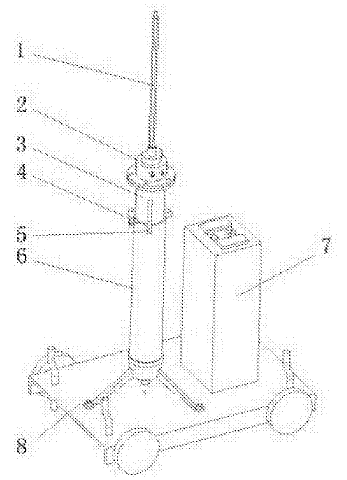
\includegraphics[width=0.5\textwidth]{IMG/driller.png}
	\bicaption[岩层信息智能钻测机]
		{岩层信息智能钻测机}
		{Intelligent drilling and measuring machine for rock stratum information}
	\label{fig:driller}
\end{figure}

该钻测机第一技术方案采用液压驱动钻杆,对钻杆提供恒定的推力和转速,测距传感器测量钻杆步进位移和速度的变化,通过这种变化判定岩层的质量状态。
	
液压驱动方面,电动机驱动定量泵运转,定量泵驱动定量马达工作,定量马达驱动钻杆钻动。
	
文献\parencite{CN107575160A}发明专利这个例子与前两者不同,该例子并未将“智能”体现在液压系统当中,其液压系统只是传动系统的一部分,其智能是工作模式、数据处理和模式识别的智能。
